% Created by tikzDevice version 0.12 on 2018-11-17 19:37:52
% !TEX encoding = UTF-8 Unicode
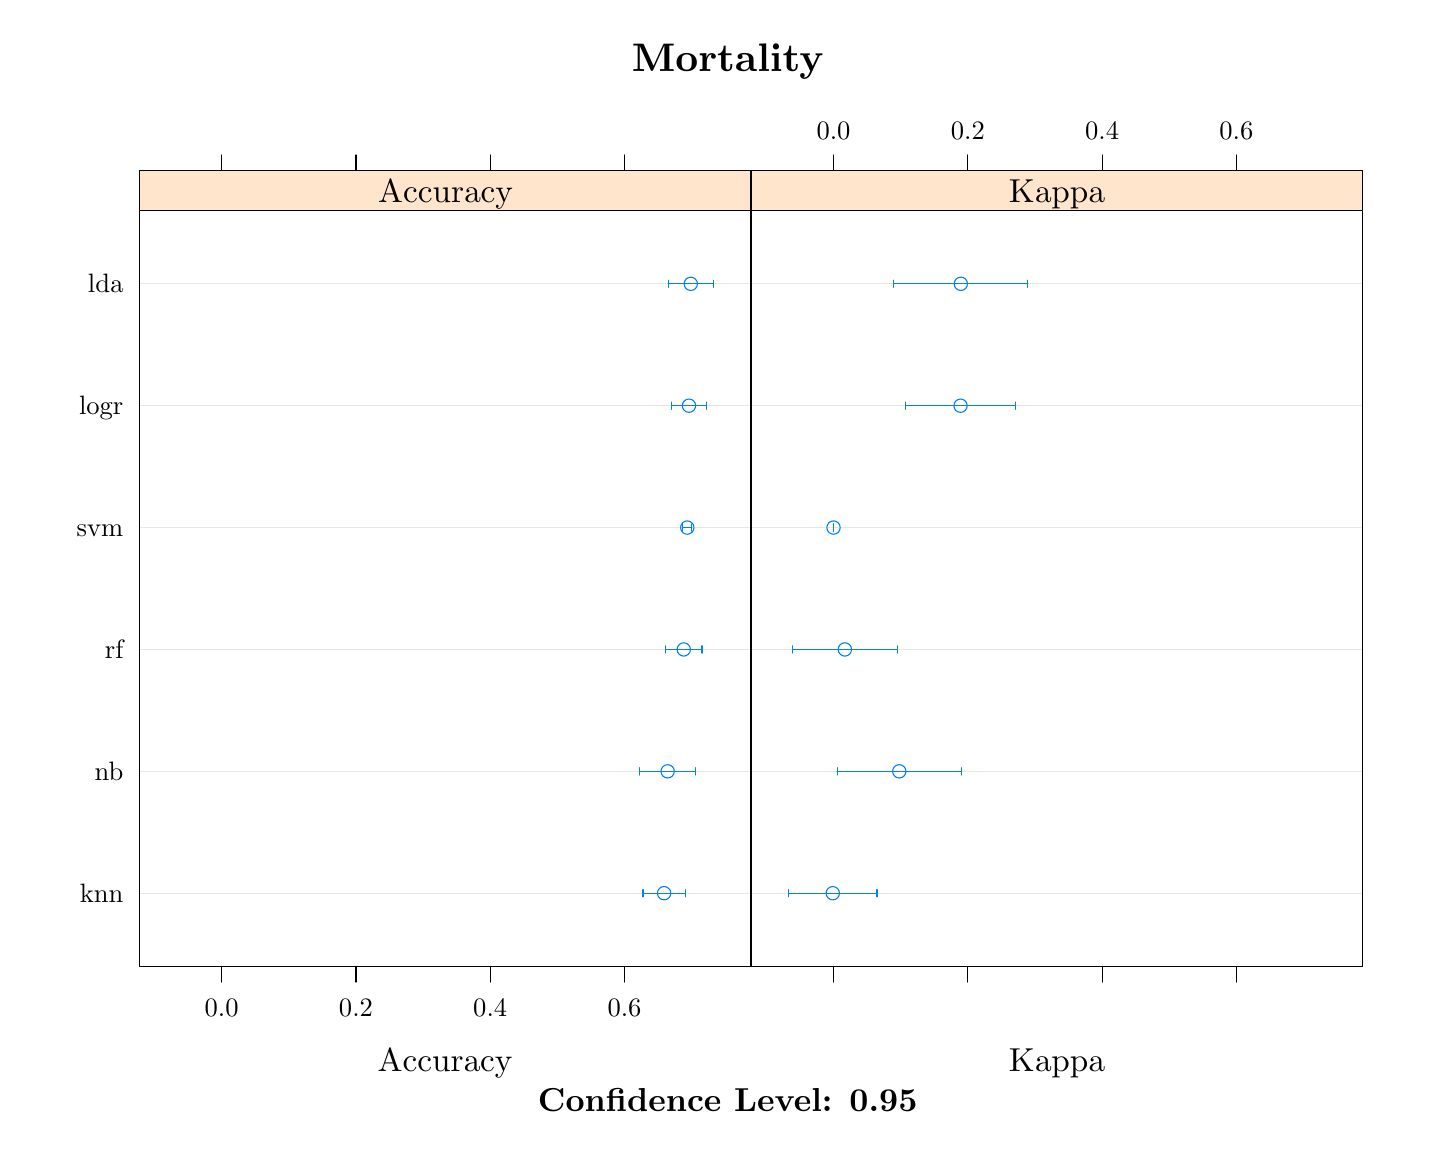
\begin{tikzpicture}[x=1pt,y=1pt]
\definecolor{fillColor}{RGB}{255,255,255}
\path[use as bounding box,fill=fillColor,fill opacity=0.00] (0,0) rectangle (505.89,397.48);
\begin{scope}
\path[clip] (  0.00,  0.00) rectangle (505.89,397.48);

\path[] (  0.00,  0.00) rectangle (505.89,397.48);
\definecolor{drawColor}{RGB}{0,0,0}

\node[text=drawColor,anchor=base,inner sep=0pt, outer sep=0pt, scale=  1.44] at (252.94,381.52) {\bfseries Mortality};
\end{scope}
\begin{scope}
\path[clip] (  0.00,  0.00) rectangle (505.89,397.48);
\definecolor{drawColor}{RGB}{0,0,0}

\node[text=drawColor,anchor=base,inner sep=0pt, outer sep=0pt, scale=  1.20] at (252.94,  6.02) {\bfseries Confidence Level: 0.95};
\end{scope}
\begin{scope}
\path[clip] (  0.00,  0.00) rectangle (505.89,397.48);
\definecolor{drawColor}{RGB}{0,0,0}

\node[text=drawColor,anchor=base,inner sep=0pt, outer sep=0pt, scale=  1.20] at (150.82, 20.33) {Accuracy};

\node[text=drawColor,anchor=base,inner sep=0pt, outer sep=0pt, scale=  1.20] at (371.92, 20.33) {Kappa};
\end{scope}
\begin{scope}
\path[clip] (  0.00,  0.00) rectangle (505.89,397.48);
\definecolor{drawColor}{RGB}{0,0,0}

\path[draw=drawColor,line width= 0.4pt,line join=round,line cap=round] ( 70.10,345.80) -- ( 70.10,351.49);

\path[draw=drawColor,line width= 0.4pt,line join=round,line cap=round] (118.62,345.80) -- (118.62,351.49);

\path[draw=drawColor,line width= 0.4pt,line join=round,line cap=round] (167.14,345.80) -- (167.14,351.49);

\path[draw=drawColor,line width= 0.4pt,line join=round,line cap=round] (215.67,345.80) -- (215.67,351.49);
\end{scope}
\begin{scope}
\path[clip] (  0.00,  0.00) rectangle (505.89,397.48);
\definecolor{drawColor}{RGB}{0,0,0}

\node[text=drawColor,anchor=base east,inner sep=0pt, outer sep=0pt, scale=  0.96] at ( 34.58, 81.41) {knn};

\node[text=drawColor,anchor=base east,inner sep=0pt, outer sep=0pt, scale=  0.96] at ( 34.58,125.45) {nb};

\node[text=drawColor,anchor=base east,inner sep=0pt, outer sep=0pt, scale=  0.96] at ( 34.58,169.49) {rf};

\node[text=drawColor,anchor=base east,inner sep=0pt, outer sep=0pt, scale=  0.96] at ( 34.58,213.53) {svm};

\node[text=drawColor,anchor=base east,inner sep=0pt, outer sep=0pt, scale=  0.96] at ( 34.58,257.57) {logr};

\node[text=drawColor,anchor=base east,inner sep=0pt, outer sep=0pt, scale=  0.96] at ( 34.58,301.61) {lda};
\end{scope}
\begin{scope}
\path[clip] (  0.00,  0.00) rectangle (505.89,397.48);
\definecolor{drawColor}{RGB}{0,0,0}

\path[draw=drawColor,line width= 0.4pt,line join=round,line cap=round] ( 70.10, 58.30) -- ( 70.10, 52.61);

\path[draw=drawColor,line width= 0.4pt,line join=round,line cap=round] (118.62, 58.30) -- (118.62, 52.61);

\path[draw=drawColor,line width= 0.4pt,line join=round,line cap=round] (167.14, 58.30) -- (167.14, 52.61);

\path[draw=drawColor,line width= 0.4pt,line join=round,line cap=round] (215.67, 58.30) -- (215.67, 52.61);

\node[text=drawColor,anchor=base,inner sep=0pt, outer sep=0pt, scale=  0.96] at ( 70.10, 40.30) {0.0};

\node[text=drawColor,anchor=base,inner sep=0pt, outer sep=0pt, scale=  0.96] at (118.62, 40.30) {0.2};

\node[text=drawColor,anchor=base,inner sep=0pt, outer sep=0pt, scale=  0.96] at (167.14, 40.30) {0.4};

\node[text=drawColor,anchor=base,inner sep=0pt, outer sep=0pt, scale=  0.96] at (215.67, 40.30) {0.6};
\end{scope}
\begin{scope}
\path[clip] ( 40.28, 58.30) rectangle (261.37,331.34);
\definecolor{drawColor}{RGB}{230,230,230}

\path[draw=drawColor,line width= 0.4pt,line join=round,line cap=round] ( 40.28, 84.72) -- (261.37, 84.72);

\path[draw=drawColor,line width= 0.4pt,line join=round,line cap=round] ( 40.28,128.76) -- (261.37,128.76);

\path[draw=drawColor,line width= 0.4pt,line join=round,line cap=round] ( 40.28,172.80) -- (261.37,172.80);

\path[draw=drawColor,line width= 0.4pt,line join=round,line cap=round] ( 40.28,216.84) -- (261.37,216.84);

\path[draw=drawColor,line width= 0.4pt,line join=round,line cap=round] ( 40.28,260.88) -- (261.37,260.88);

\path[draw=drawColor,line width= 0.4pt,line join=round,line cap=round] ( 40.28,304.92) -- (261.37,304.92);
\definecolor{drawColor}{RGB}{0,128,255}

\path[draw=drawColor,line width= 0.4pt,line join=round,line cap=round] (229.97, 84.72) circle (  2.41);

\path[draw=drawColor,line width= 0.4pt,line join=round,line cap=round] (231.25,128.76) circle (  2.41);

\path[draw=drawColor,line width= 0.4pt,line join=round,line cap=round] (237.07,172.80) circle (  2.41);

\path[draw=drawColor,line width= 0.4pt,line join=round,line cap=round] (238.34,216.84) circle (  2.41);

\path[draw=drawColor,line width= 0.4pt,line join=round,line cap=round] (238.96,260.88) circle (  2.41);

\path[draw=drawColor,line width= 0.4pt,line join=round,line cap=round] (239.60,304.92) circle (  2.41);

\path[draw=drawColor,line width= 0.4pt,line join=round,line cap=round] (222.36, 84.72) -- (237.59, 84.72);

\path[draw=drawColor,line width= 0.4pt,line join=round,line cap=round] (221.19,128.76) -- (241.31,128.76);

\path[draw=drawColor,line width= 0.4pt,line join=round,line cap=round] (230.47,172.80) -- (243.66,172.80);

\path[draw=drawColor,line width= 0.4pt,line join=round,line cap=round] (236.65,216.84) -- (240.03,216.84);

\path[draw=drawColor,line width= 0.4pt,line join=round,line cap=round] (232.76,260.88) -- (245.17,260.88);

\path[draw=drawColor,line width= 0.4pt,line join=round,line cap=round] (231.41,304.92) -- (247.79,304.92);

\path[draw=drawColor,line width= 0.4pt,line join=round,line cap=round] (222.36, 86.04) -- (222.36, 83.40);

\path[draw=drawColor,line width= 0.4pt,line join=round,line cap=round] (221.19,130.08) -- (221.19,127.44);

\path[draw=drawColor,line width= 0.4pt,line join=round,line cap=round] (230.47,174.12) -- (230.47,171.48);

\path[draw=drawColor,line width= 0.4pt,line join=round,line cap=round] (236.65,218.16) -- (236.65,215.52);

\path[draw=drawColor,line width= 0.4pt,line join=round,line cap=round] (232.76,262.20) -- (232.76,259.56);

\path[draw=drawColor,line width= 0.4pt,line join=round,line cap=round] (231.41,306.24) -- (231.41,303.60);

\path[draw=drawColor,line width= 0.4pt,line join=round,line cap=round] (237.59, 86.04) -- (237.59, 83.40);

\path[draw=drawColor,line width= 0.4pt,line join=round,line cap=round] (241.31,130.08) -- (241.31,127.44);

\path[draw=drawColor,line width= 0.4pt,line join=round,line cap=round] (243.66,174.12) -- (243.66,171.48);

\path[draw=drawColor,line width= 0.4pt,line join=round,line cap=round] (240.03,218.16) -- (240.03,215.52);

\path[draw=drawColor,line width= 0.4pt,line join=round,line cap=round] (245.17,262.20) -- (245.17,259.56);

\path[draw=drawColor,line width= 0.4pt,line join=round,line cap=round] (247.79,306.24) -- (247.79,303.60);
\end{scope}
\begin{scope}
\path[clip] (  0.00,  0.00) rectangle (505.89,397.48);
\definecolor{drawColor}{RGB}{0,0,0}

\path[draw=drawColor,line width= 0.4pt,line join=round,line cap=round] ( 40.28, 58.30) rectangle (261.37,331.34);
\end{scope}
\begin{scope}
\path[clip] ( 40.28,331.34) rectangle (261.37,345.80);
\definecolor{drawColor}{RGB}{255,229,204}
\definecolor{fillColor}{RGB}{255,229,204}

\path[draw=drawColor,line width= 0.4pt,line join=round,line cap=round,fill=fillColor] ( 40.28,331.34) rectangle (261.37,345.80);
\definecolor{drawColor}{RGB}{0,0,0}

\node[text=drawColor,anchor=base west,inner sep=0pt, outer sep=0pt, scale=  1.20] at (126.65,334.44) {Accuracy};
\end{scope}
\begin{scope}
\path[clip] (  0.00,  0.00) rectangle (505.89,397.48);
\definecolor{drawColor}{RGB}{0,0,0}

\path[draw=drawColor,line width= 0.4pt,line join=round,line cap=round] ( 40.28,331.34) rectangle (261.37,345.80);
\end{scope}
\begin{scope}
\path[clip] (  0.00,  0.00) rectangle (505.89,397.48);
\definecolor{drawColor}{RGB}{0,0,0}

\path[draw=drawColor,line width= 0.4pt,line join=round,line cap=round] (291.19,345.80) -- (291.19,351.49);

\path[draw=drawColor,line width= 0.4pt,line join=round,line cap=round] (339.72,345.80) -- (339.72,351.49);

\path[draw=drawColor,line width= 0.4pt,line join=round,line cap=round] (388.24,345.80) -- (388.24,351.49);

\path[draw=drawColor,line width= 0.4pt,line join=round,line cap=round] (436.76,345.80) -- (436.76,351.49);

\node[text=drawColor,anchor=base,inner sep=0pt, outer sep=0pt, scale=  0.96] at (291.19,357.18) {0.0};

\node[text=drawColor,anchor=base,inner sep=0pt, outer sep=0pt, scale=  0.96] at (339.72,357.18) {0.2};

\node[text=drawColor,anchor=base,inner sep=0pt, outer sep=0pt, scale=  0.96] at (388.24,357.18) {0.4};

\node[text=drawColor,anchor=base,inner sep=0pt, outer sep=0pt, scale=  0.96] at (436.76,357.18) {0.6};
\end{scope}
\begin{scope}
\path[clip] (  0.00,  0.00) rectangle (505.89,397.48);
\definecolor{drawColor}{RGB}{0,0,0}

\path[draw=drawColor,line width= 0.4pt,line join=round,line cap=round] (291.19, 58.30) -- (291.19, 52.61);

\path[draw=drawColor,line width= 0.4pt,line join=round,line cap=round] (339.72, 58.30) -- (339.72, 52.61);

\path[draw=drawColor,line width= 0.4pt,line join=round,line cap=round] (388.24, 58.30) -- (388.24, 52.61);

\path[draw=drawColor,line width= 0.4pt,line join=round,line cap=round] (436.76, 58.30) -- (436.76, 52.61);
\end{scope}
\begin{scope}
\path[clip] (261.37, 58.30) rectangle (482.46,331.34);
\definecolor{drawColor}{RGB}{230,230,230}

\path[draw=drawColor,line width= 0.4pt,line join=round,line cap=round] (261.37, 84.72) -- (482.46, 84.72);

\path[draw=drawColor,line width= 0.4pt,line join=round,line cap=round] (261.37,128.76) -- (482.46,128.76);

\path[draw=drawColor,line width= 0.4pt,line join=round,line cap=round] (261.37,172.80) -- (482.46,172.80);

\path[draw=drawColor,line width= 0.4pt,line join=round,line cap=round] (261.37,216.84) -- (482.46,216.84);

\path[draw=drawColor,line width= 0.4pt,line join=round,line cap=round] (261.37,260.88) -- (482.46,260.88);

\path[draw=drawColor,line width= 0.4pt,line join=round,line cap=round] (261.37,304.92) -- (482.46,304.92);
\definecolor{drawColor}{RGB}{0,128,255}

\path[draw=drawColor,line width= 0.4pt,line join=round,line cap=round] (290.92, 84.72) circle (  2.41);

\path[draw=drawColor,line width= 0.4pt,line join=round,line cap=round] (314.95,128.76) circle (  2.41);

\path[draw=drawColor,line width= 0.4pt,line join=round,line cap=round] (295.29,172.80) circle (  2.41);

\path[draw=drawColor,line width= 0.4pt,line join=round,line cap=round] (291.19,216.84) circle (  2.41);

\path[draw=drawColor,line width= 0.4pt,line join=round,line cap=round] (337.09,260.88) circle (  2.41);

\path[draw=drawColor,line width= 0.4pt,line join=round,line cap=round] (337.18,304.92) circle (  2.41);

\path[draw=drawColor,line width= 0.4pt,line join=round,line cap=round] (274.95, 84.72) -- (306.89, 84.72);

\path[draw=drawColor,line width= 0.4pt,line join=round,line cap=round] (292.52,128.76) -- (337.38,128.76);

\path[draw=drawColor,line width= 0.4pt,line join=round,line cap=round] (276.41,172.80) -- (314.17,172.80);

\path[draw=drawColor,line width= 0.4pt,line join=round,line cap=round] (291.19,216.84) -- (291.19,216.84);

\path[draw=drawColor,line width= 0.4pt,line join=round,line cap=round] (317.27,260.88) -- (356.90,260.88);

\path[draw=drawColor,line width= 0.4pt,line join=round,line cap=round] (312.95,304.92) -- (361.41,304.92);

\path[draw=drawColor,line width= 0.4pt,line join=round,line cap=round] (274.95, 86.04) -- (274.95, 83.40);

\path[draw=drawColor,line width= 0.4pt,line join=round,line cap=round] (292.52,130.08) -- (292.52,127.44);

\path[draw=drawColor,line width= 0.4pt,line join=round,line cap=round] (276.41,174.12) -- (276.41,171.48);

\path[draw=drawColor,line width= 0.4pt,line join=round,line cap=round] (291.19,218.16) -- (291.19,215.52);

\path[draw=drawColor,line width= 0.4pt,line join=round,line cap=round] (317.27,262.20) -- (317.27,259.56);

\path[draw=drawColor,line width= 0.4pt,line join=round,line cap=round] (312.95,306.24) -- (312.95,303.60);

\path[draw=drawColor,line width= 0.4pt,line join=round,line cap=round] (306.89, 86.04) -- (306.89, 83.40);

\path[draw=drawColor,line width= 0.4pt,line join=round,line cap=round] (337.38,130.08) -- (337.38,127.44);

\path[draw=drawColor,line width= 0.4pt,line join=round,line cap=round] (314.17,174.12) -- (314.17,171.48);

\path[draw=drawColor,line width= 0.4pt,line join=round,line cap=round] (291.19,218.16) -- (291.19,215.52);

\path[draw=drawColor,line width= 0.4pt,line join=round,line cap=round] (356.90,262.20) -- (356.90,259.56);

\path[draw=drawColor,line width= 0.4pt,line join=round,line cap=round] (361.41,306.24) -- (361.41,303.60);
\end{scope}
\begin{scope}
\path[clip] (  0.00,  0.00) rectangle (505.89,397.48);
\definecolor{drawColor}{RGB}{0,0,0}

\path[draw=drawColor,line width= 0.4pt,line join=round,line cap=round] (261.37, 58.30) rectangle (482.46,331.34);
\end{scope}
\begin{scope}
\path[clip] (261.37,331.34) rectangle (482.46,345.80);
\definecolor{drawColor}{RGB}{255,229,204}
\definecolor{fillColor}{RGB}{255,229,204}

\path[draw=drawColor,line width= 0.4pt,line join=round,line cap=round,fill=fillColor] (261.37,331.34) rectangle (482.46,345.80);
\definecolor{drawColor}{RGB}{0,0,0}

\node[text=drawColor,anchor=base west,inner sep=0pt, outer sep=0pt, scale=  1.20] at (354.59,334.44) {Kappa};
\end{scope}
\begin{scope}
\path[clip] (  0.00,  0.00) rectangle (505.89,397.48);
\definecolor{drawColor}{RGB}{0,0,0}

\path[draw=drawColor,line width= 0.4pt,line join=round,line cap=round] (261.37,331.34) rectangle (482.46,345.80);
\end{scope}
\end{tikzpicture}
